
\section{Réglage de la position d'équilibre du pendule \label{ccmp2023_sec_02}}
Comme pour les applications terrestres, chaque système du sismomètre VBB possède un pendule qui oscille par rapport à un bâti sous l'impulsion de secousses sismiques transmises par le sol à l'instrument. Une articulation à lamelles permet des mouvements de très faible amplitude avec un minimum de frottements visqueux entre le pendule et le bâti, et sans jeu. Elle constitue l'axe de rotation du pendule dans son mouvement par rapport au bâti.

Le sismomètre VBB s'appuie sur le principe du pendule inversé. L'instabilité inhérente au pendule inversé lui confère une plus grande sensibilité que celle d'un pendule classique. Bien qu'instable par nature, le pendule inversé du sismomètre VBB conserve son équilibre grâce à un ressort à lame souple, recourbé en demi-cercle, et qui applique en permanence une action mécanique de rappel.

\subsection{Compensation de la gravité terrestre \label{ccmp2023_sec_02_01}}
Le sismomètre étant optimisé pour fonctionner sous gravité martienne, il n'est pas possible de le tester sur Terre sans y apporter des modifications. En effet, pour un mouvement du sol donné sur Terre, l'amplitude résultante des oscillations du pendule risquerait de détériorer le mécanisme. Un contrepoids est ajouté au pendule, dont le moment généré sur son axe de rotation par rapport au bâti doit compenser celui dû à la différence de gravité entre la Terre et Mars (voir figure \ref{ccmp2023_fig_03b}).



\begin{figure*}[h!]
    \centering
    \begin{subfigure}[t]{0.45\textwidth}
        \centering
        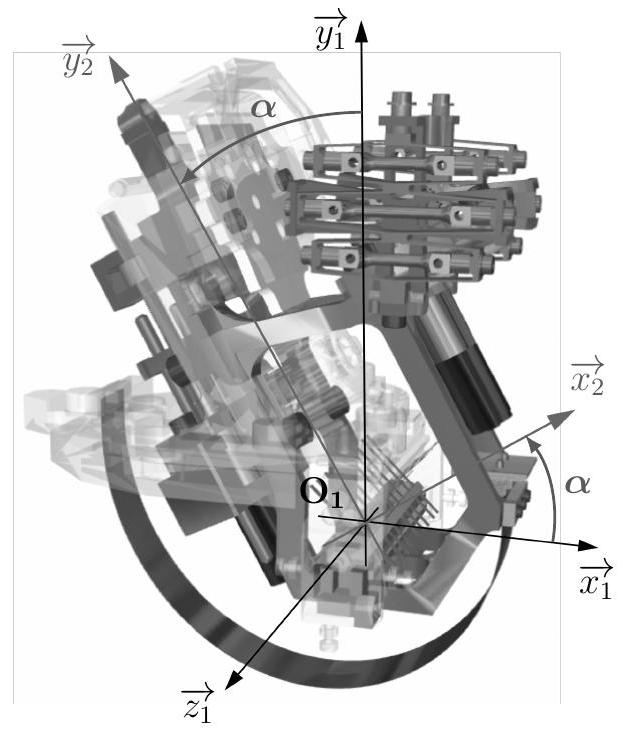
\includegraphics[height=5.5cm]{2024_04_26_3285cfc264024262add0g-04}
        \caption{\label{ccmp2023_fig_03a} Pendule en niveaux de gris; bâti en transparence (voir aussi Annexe 1).}
    \end{subfigure}%
    \hfill
    \begin{subfigure}[t]{0.45\textwidth}
        \centering
        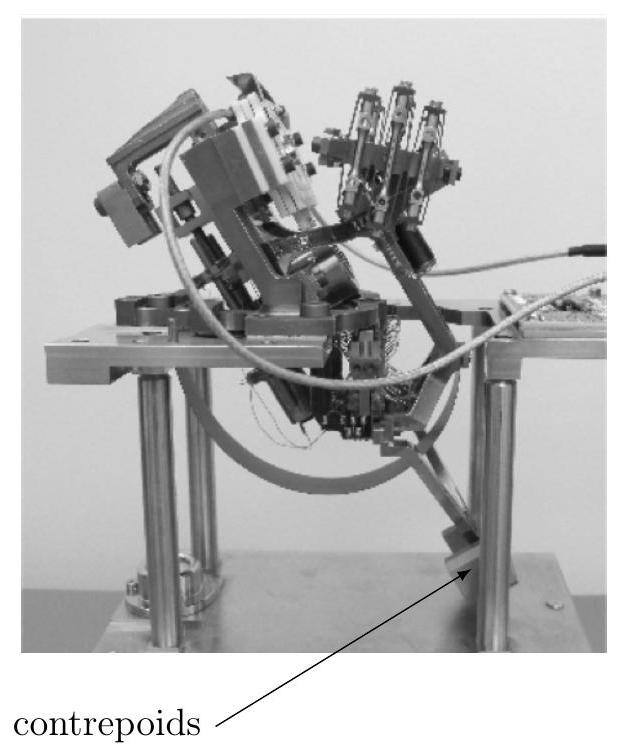
\includegraphics[height=5.5cm]{2024_04_26_3285cfc264024262add0g-04(1)}
        \caption{\label{ccmp2023_fig_03b} Dispositif expérimental avec contrepoids pour tester les oscillations du pendule sur Terre}
    \end{subfigure}
    \caption{}
\end{figure*}


%
%\begin{figure}[!h]
%\centering
%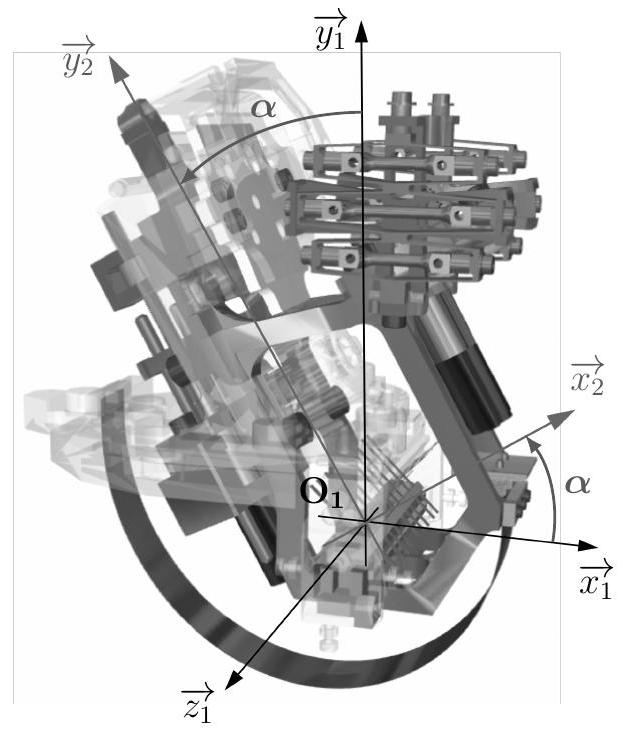
\includegraphics[width=\textwidth]{2024_04_26_3285cfc264024262add0g-04}
%\caption{\label{ccmp2023_fig_03}(a) Pendule en niveaux de gris; bâti en transparence (voir aussi Annexe 1).}
%%
%\end{figure}
%
%(a) Pendule en niveaux de gris; bâti en transparence (voir aussi Annexe 1).
%
%\begin{figure}[!h]
%\centering
%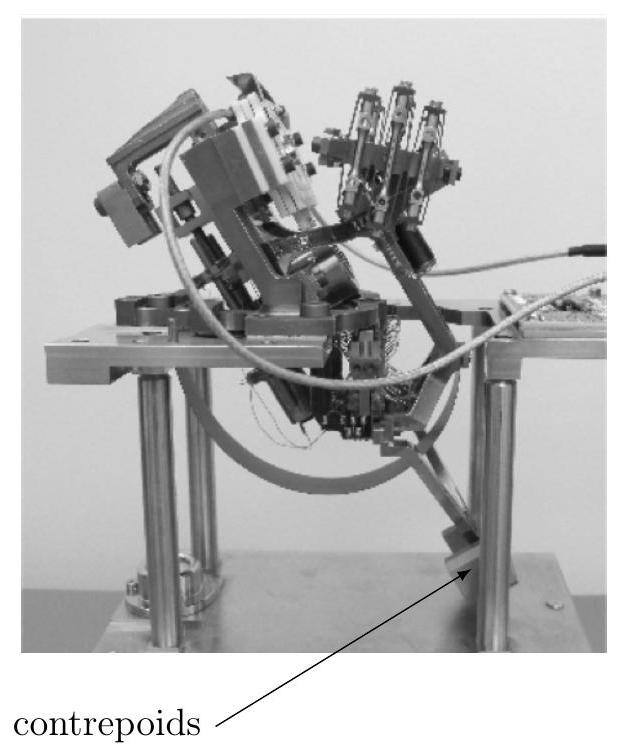
\includegraphics[width=\textwidth]{2024_04_26_3285cfc264024262add0g-04(1)}
%\caption{\label{ccmp2023_fig_01}
%\end{center}
%
%(b) Dispositif expérimental avec contrepoids pour tester les oscillations du pendule sur Terre
%
%FIGURE 3



\begin{obj}
Etablir les conditions que doit respecter le contrepoids pour compenser la gravité terrestre lors d'expériences sur Terre.
\end{obj}
 

Le schéma cinématique et le paramétrage du dispositif sont fournis en Annexe 2, ainsi que l'ensemble des notations et hypothèses utiles pour cette sous-partie.

On désigne par «~ensemble mobile~» le pendule noté (2) équipé du contrepoids noté (3). Le bâti, lié au sol, est noté~(1).

\question{\label{ccmp2023_q_01}Écrire l'équation traduisant l'équilibre de l'ensemble mobile $\{(2)+(3)\}$ sur Terre, lorsque $\alpha(t)=\alpha_{\mathrm{eq}}$. Préciser le bilan des actions mécaniques extérieures, le théorème ou principe utilisé, et les éléments d'application (projection, point éventuel).}

Sur Mars, le pendule (2) n'est pas équipé du contrepoids (3). Cependant, la position d'équilibre du pendule (2) sans contrepoids (3) sur Mars, et celle du pendule (2) avec le contrepoids (3) sur Terre, doivent être identiques.

\question{\label{ccmp2023_q_02}Donner la condition sur la masse $m_{3}$ et la variable $b$ pour compenser la différence de pesanteur entre la Terre et Mars. Pour cela, exprimer le produit $b m_{3}$ en fonction de $a$, $M_{2}, g_{T}$ et $g_{M}$.}

Cette condition étant respectée, on peut alors traduire l'équilibre de l'ensemble mobile sur Terre :


$$
a M_{2} g_{\mathrm{M}} \sin \alpha_{\mathrm{eq}}+C_{0}-k\left(\alpha_{\mathrm{eq}}-\alpha_{0}\right)=0 %\tag{eq.1}
$$


\subsection{Conception d'un mécanisme de translation du centre d'inertie du pendule}
Si l'inclinaison de la surface sur laquelle le sismomètre est posé n'est pas correctement corrigée par les pieds réglables, la position $a$ du centre d'inertie $G_{2}$ du pendule (2) le long de l'axe $\left(O_{1}, \overrightarrow{y_{2}}\right)$ peut être réglée à distance. Cela permet notamment d'assurer que $\alpha_{\mathrm{eq}}$ conserve une valeur optimale déterminée lors d'expérimentations sur Terre.

Pour cela, un mécanisme embarqué sur (2), constitué d'un moteur pas-à-pas, d'un réducteur à train épicycloïdal, d'un joint d'accouplement (joint d'Oldham) et d'un système vis-écrou, indiqués enfigure \label{ccmp2023_fig_04}, est guidé en translation le long de l'axe  $\axe{O_1}{y_2}$.

\begin{obj}
Justifier les choix de conception du mécanisme de translation du centre d'inertie du pendule.
\end{obj}

%\begin{figure}[!h]
%\centering
%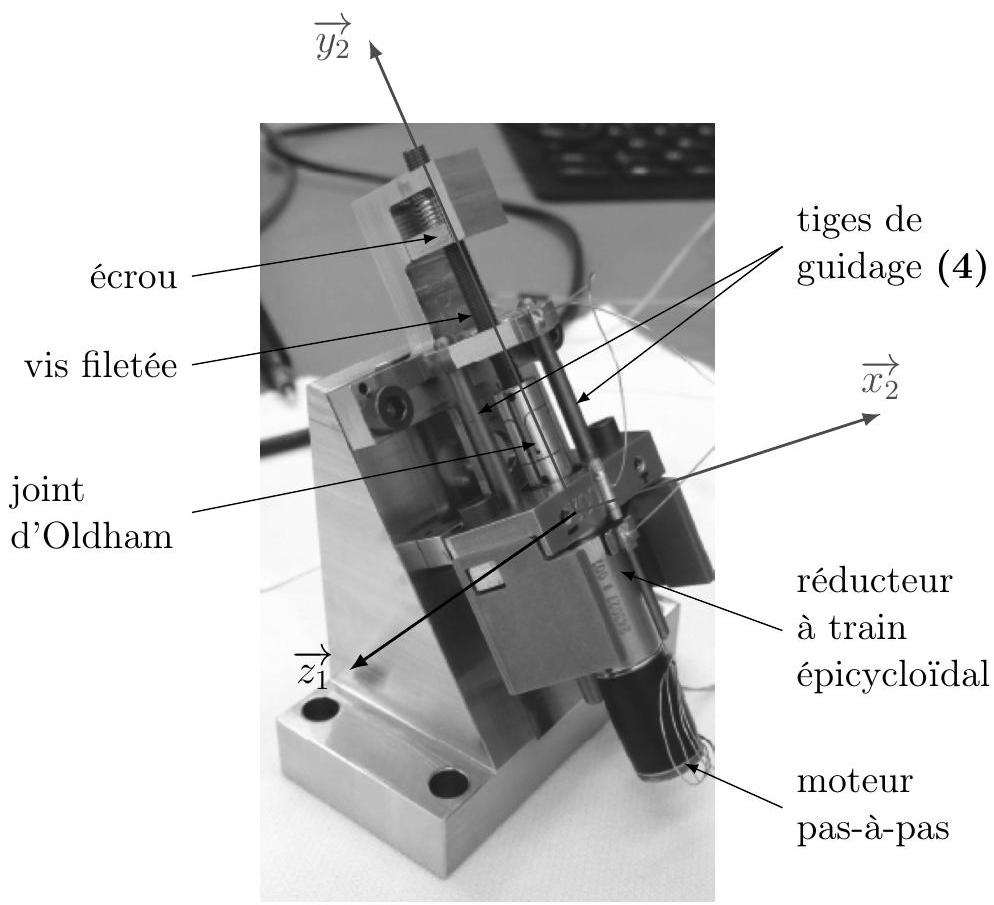
\includegraphics[width=\textwidth]{2024_04_26_3285cfc264024262add0g-05(1)}
%\caption{\label{ccmp2023_fig_04} Photographie du mécanisme de réglage de la position du centre d'inertie du pendule. Le mécanisme est ici fixé sur un support métallique incliné représentant le corps du pendule (2).}
%% FiguRe 4 - Photographie du mécanisme de réglage de la position du centre d'inertie du pendule. Le mécanisme est ici fixé sur un support métallique incliné représentant le corps du pendule (2).
%\end{figure}


\begin{minipage}[c]{.45\linewidth}
    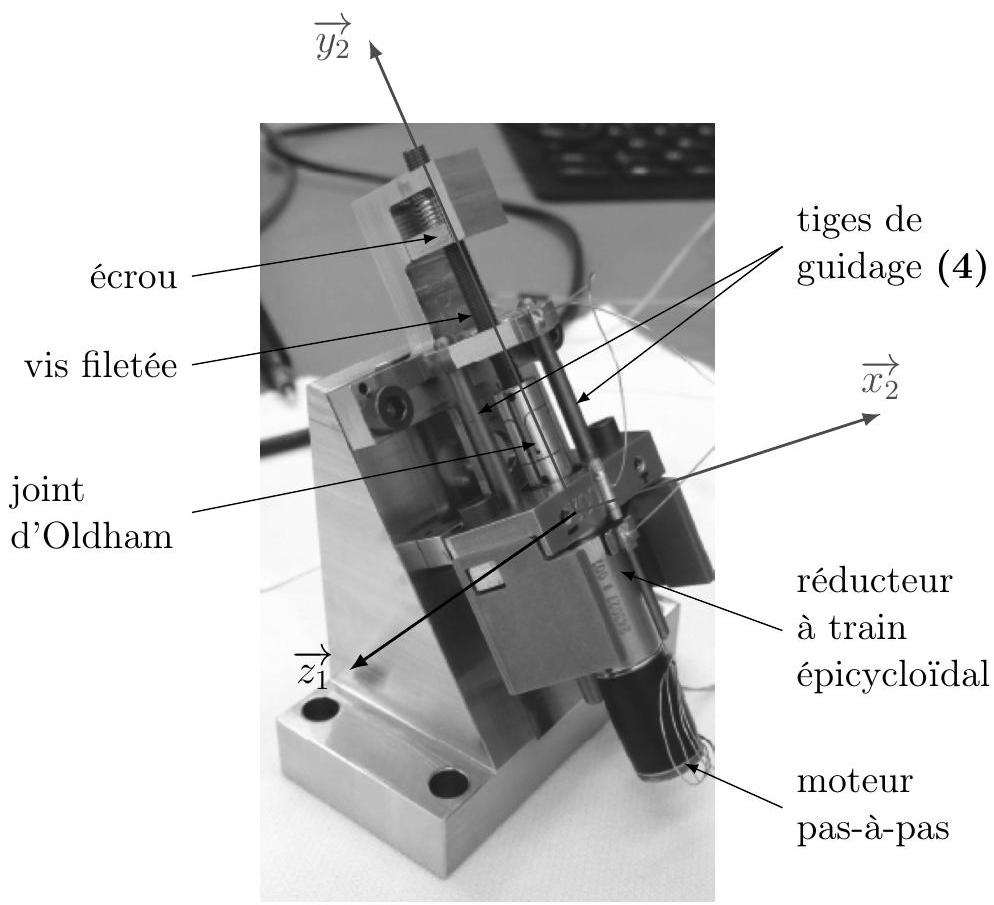
\includegraphics[height=6.5cm]{2024_04_26_3285cfc264024262add0g-05(1)}
    \captionof{figure} {\label{ccmp2023_fig_04} Photographie du mécanisme de réglage de la position du centre d'inertie du pendule. Le mécanisme est ici fixé sur un support métallique incliné représentant le corps du pendule (2).}
\end{minipage}
\hfill
\begin{minipage}[c]{.45\linewidth}
        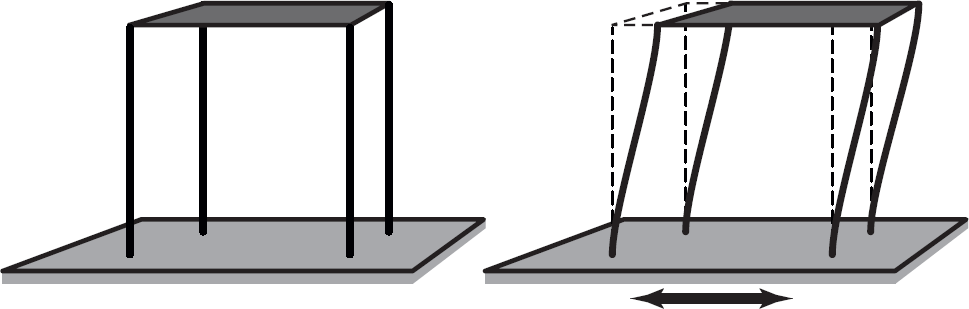
\includegraphics[height=5.5cm]{fig_05}
        \captionof{figure} {\label{ccmp2023_fig_05} Schéma cinématique du guidage en translation des tiges (4) par rapport au corps du pendule (2)}
\end{minipage}


Pendant la phase de réglage de la position de son centre d'inertie, on suppose que le corps du pendule (2) reste immobile. L'ensemble du mécanisme embarqué est considéré comme mobile par rapport au corps du pendule (2) le temps de cette étude.

Le guidage en translation des tiges (4) par rapport à (2) permettant le réglage de la position du centre d'inertie est réalisé par l'association de 4 liaisons en parallèle (voir figure \label{ccmp2023_fig_05}).


%Q3. 
\question{\label{ccmp2023_q_03}Compléter, sur le Cahier Réponses, le graphe des liaisons fourni avec les noms et la (les) caractéristique(s) géométrique(s) des liaisons. Donner le nombre de boucles indépendantes (nombre cyclomatique $\gamma$ ) de ce modèle.}

\question{\label{ccmp2023_q_04}Déterminer le degré d'hyperstatisme $h$ de ce modèle. Préciser les mobilités internes $\left(m_{i}\right)$ et utiles $\left(m_{u}\right)$. Justifier, au regard du système et de son contexte d'utilisation, l'intérêt d'un tel degré d'hyperstatisme pour la réalisation du guidage.}

L'association des 4 liaisons en parallèle entre (4) et (2) correspond à une liaison glissière équivalente de direction $\overrightarrow{y_{2}}$. La suite de l'étude s'appuiera sur le schéma cinématique réduit de la figure \label{ccmp2023_fig_06} faisant apparaître cette liaison équivalente, ainsi que des éléments du mécanisme embarqué. Le schéma cinématique réduit de l'ensemble du mécanisme est fourni en Annexe 3.

Le joint de type Oldham assure l'accouplement de l'arbre (5) en sortie du réducteur à train épicycloïdal avec la vis (v).

La figure \label{ccmp2023_fig_07} présente les éléments constitutifs d'un joint d'Oldham :

\begin{itemize}
  \item le plateau d'entrée est cinématiquement lié à l'arbre (5) en sortie du réducteur;
  \item le plateau de sortie est cinématiquement lié à la vis (v);
  \item la noix, repérée $(\mathbf{N})$, est la pièce intermédiaire du joint.
\end{itemize}

On suppose que le joint est assemblé sans jeu entre les différentes surfaces de contact.

\begin{figure}[!h]
\centering
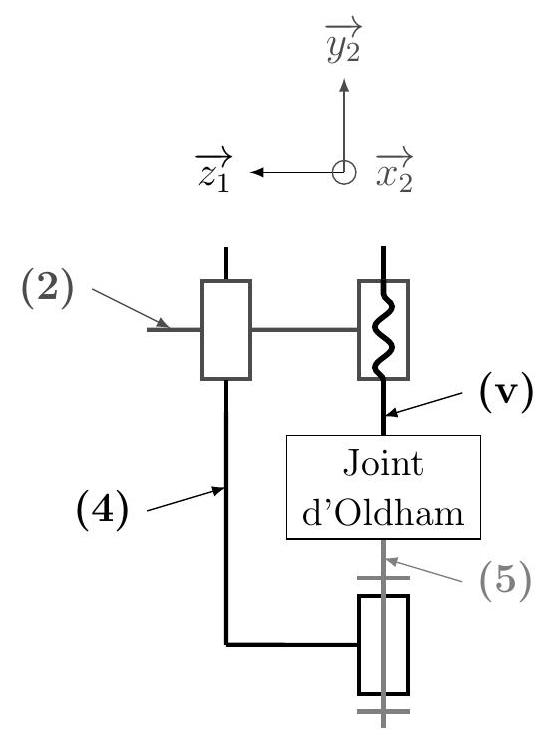
\includegraphics[width=4cm]{2024_04_26_3285cfc264024262add0g-06(1)}
\caption{\label{ccmp2023_fig_06} Schéma cinématique réduit du mécanisme de déplacement du centre d'inertie du pendule}
%FigURE 6 - Schéma cinématique réduit du mécanisme de déplacement du centre d'inertie du pendule\\
\end{figure}

\begin{figure}[!h]
\centering
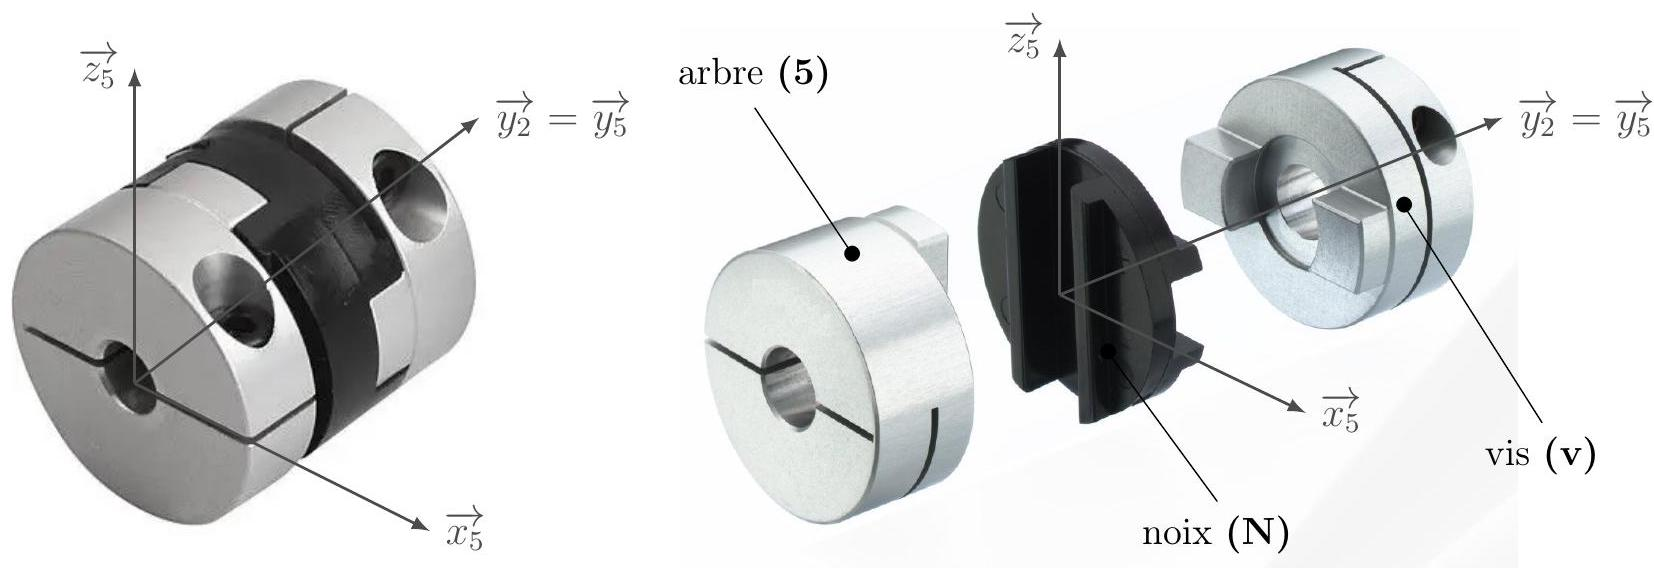
\includegraphics[width=\textwidth]{2024_04_26_3285cfc264024262add0g-06}
\caption{\label{ccmp2023_fig_07} Joint d'Oldham assemblé (à gauche) et éclaté (à droite)}
%FiguRe 7 - Joint d'Oldham assemblé (à gauche) et éclaté (à droite)
\end{figure}


%Q5. 
\question{\label{ccmp2023_q_05}À l'aide de la figure \ref{ccmp2023_fig_07} et par analyse des surfaces de contact, identifier la liaison entre $(\mathbf{N})$ et (5) d'une part, et entre (N) et (v) d'autre part. Compléter le schéma cinématique en 3D du Cahier Réponses en traçant ces liaisons.}

Ce type de joint permet de lier entre eux des éléments d'un mécanisme tout en corrigeant d'éventuels défauts de positionnement relatif entre les arbres (5) et (v).

%}Q6. 
\question{\label{ccmp2023_q_06} Pour chacune des 5 propositions de défauts géométriques du tableau du Cahier Réponses, entourer OUI lorsque le joint d'Oldham permet de rattraper le défaut et entourer NON lorsque ce n'est pas le cas.}



\subsection{Validation de la précision du positionnement du centre d'inertie du pendule}

\begin{table}[!h]
\centering
\begin{tabular}{llll}
\hline
Id & Exigence & Critère & Niveau \\
\hline
$\mathbf{1}$ & Ajuster la position d'équilibre du pendule sur Mars &  &  \\
\hline
$\mathbf{1 . 1}$ & Déplacer le centre d'inertie du pendule & Précision du positionnement & $\pm 3 \mu \mathrm{m}$ \\
\hline
\end{tabular}
\caption{\label{ccmp2023_tab_01} Liste (non exhaustive) des exigences du mécanisme de translation du centre d'inertie du pendule}
%TABLE 1 - Liste (non exhaustive) des exigences du mécanisme de translation du centre d'inertie du pendule
\end{table}

\begin{obj}
Vérifier que l'exigence 1.1 de précision du positionnement du centre d'inertie du pendule est bien validée.
\end{obj}

On introduit, pour le vecteur vitesse de rotation d'un solide $i$ par rapport à un solide $j$, la notation suivante :

$$
\vec{\Omega}_{i / j} \cdot \overrightarrow{y_{2}}=\omega_{i / j}
$$

Les éléments du mécanisme de transformation de mouvement permettant le déplacement du centre d'inertie du pendule sont rappelés en figure \ref{ccmp2023_fig_08}. Leurs caractéristiques y sont précisées.

\begin{figure}[!h]
\centering
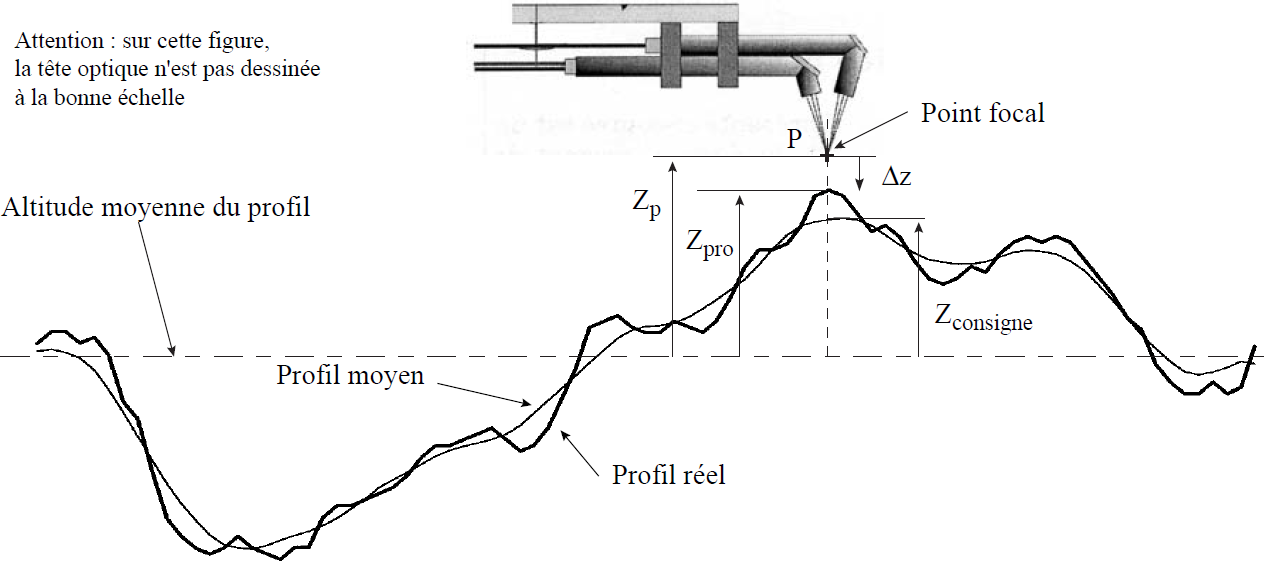
\includegraphics[width=\textwidth]{fig_08}
\caption{\label{ccmp2023_fig_08} Chaîne de transmission réalisant le déplacement de la position du centre d'inertie du pendule}
%FigURE 8 - Chaîne de transmission réalisant le déplacement de la position du centre d'inertie du pendule
\end{figure}


%FigURE 8 - Chaîne de transmission réalisant le déplacement de la position du centre d'inertie du pendule

Le joint d'Oldham est homocinétique, c'est-à-dire que la vitesse de rotation de l'arbre de sortie du réducteur (5) est la même que celle de la vis (v) par rapport au pendule (2) :

$$
\omega_{5 / 2}=\omega_{v / 2}
$$

Le réducteur est à train épicycloïdal. Son schéma complet est fourni en Annexe 3. Comme il est composé de 4 étages identiques, on résume son étude à celle d'un seul étage, ici le dernier, de manière à en déduire par la suite le rapport de transmission global du train complet. Le schéma cinématique du dernier étage du réducteur est fourni en figure \ref{ccmp2023_fig_09}.


\question{\label{ccmp2023_q_07}Justifier que $\omega_{4 / 2}=0$. Établir l'expression du rapport de transmission d'un étage $k=\frac{\omega_{5 / 2}}{\omega_{7 / 2}}$ en fonction des nombres de dents $Z_{i}$ et faire l'application numérique.}


\begin{figure}[!h]
\centering
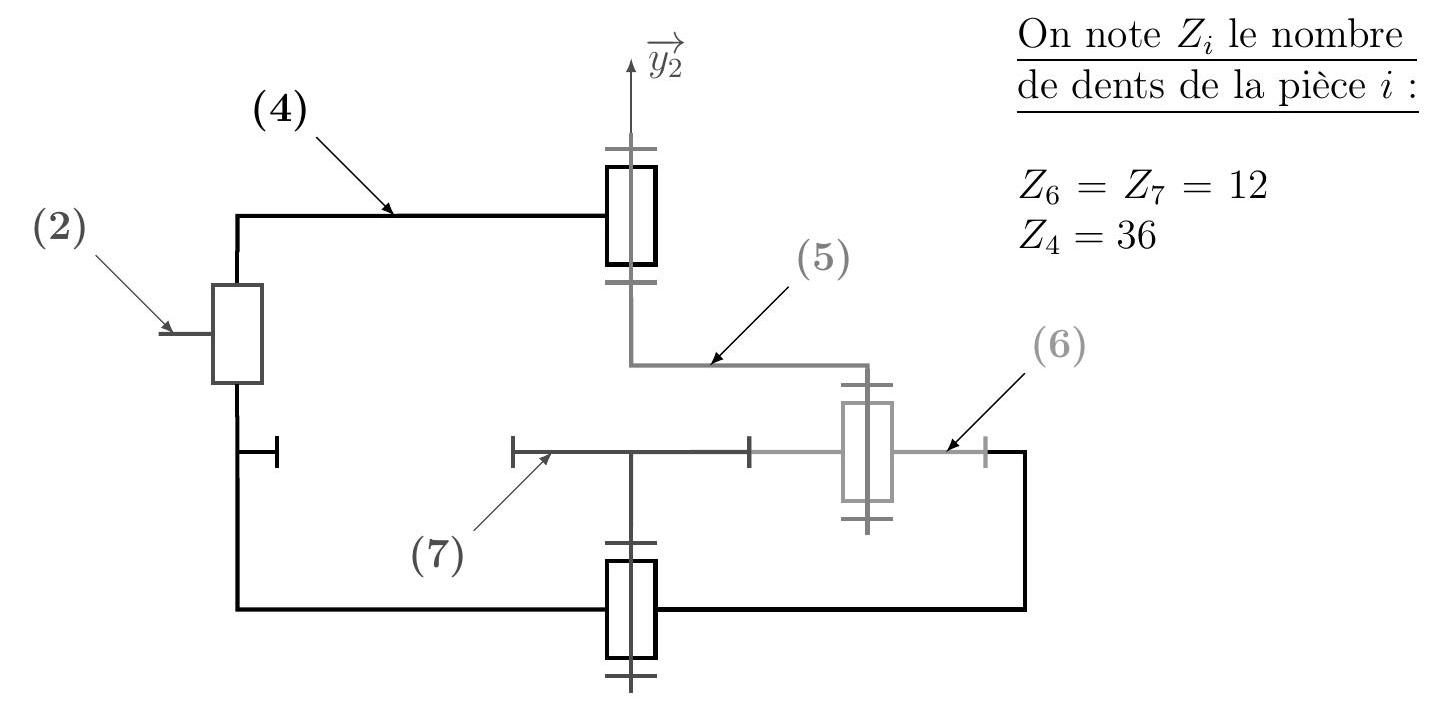
\includegraphics[width=.7\textwidth]{2024_04_26_3285cfc264024262add0g-08}
\caption{\label{ccmp2023_fig_09} Schéma cinématique du dernier étage du train épicycloïdal}
%FigURe 9 - Schéma cinématique du dernier étage du train épicycloïdal
\end{figure}


%Q08
\question{\label{ccmp2023_q_08}Exprimer le rapport de transmission global du réducteur $k_{g}=\frac{\omega_{5 / 2}}{\omega_{m / 2}}$ en fonction de $k$.}

\question{\label{ccmp2023_q_09}En s'appuyant sur les notations et données de la figure \ref{ccmp2023_fig_08}, établir l'expression du déplacement linéaire $d_{v}$ de la vis (v) par pas du moteur en fonction de $N_{m}, k_{g}$ et $p_{v}$. Faire l'application numérique et conclure vis-à-vis de l'exigence 1.1 de précision du positionnement du centre d'inertie.}

Un capteur optique a permis de mesurer le déplacement de la vis, fourni en figure \ref{ccmp2023_fig_10}, et a mis en évidence une non-linéarité lors des changements de sens de rotation du moteur.\\

\begin{figure}[!h]
\centering
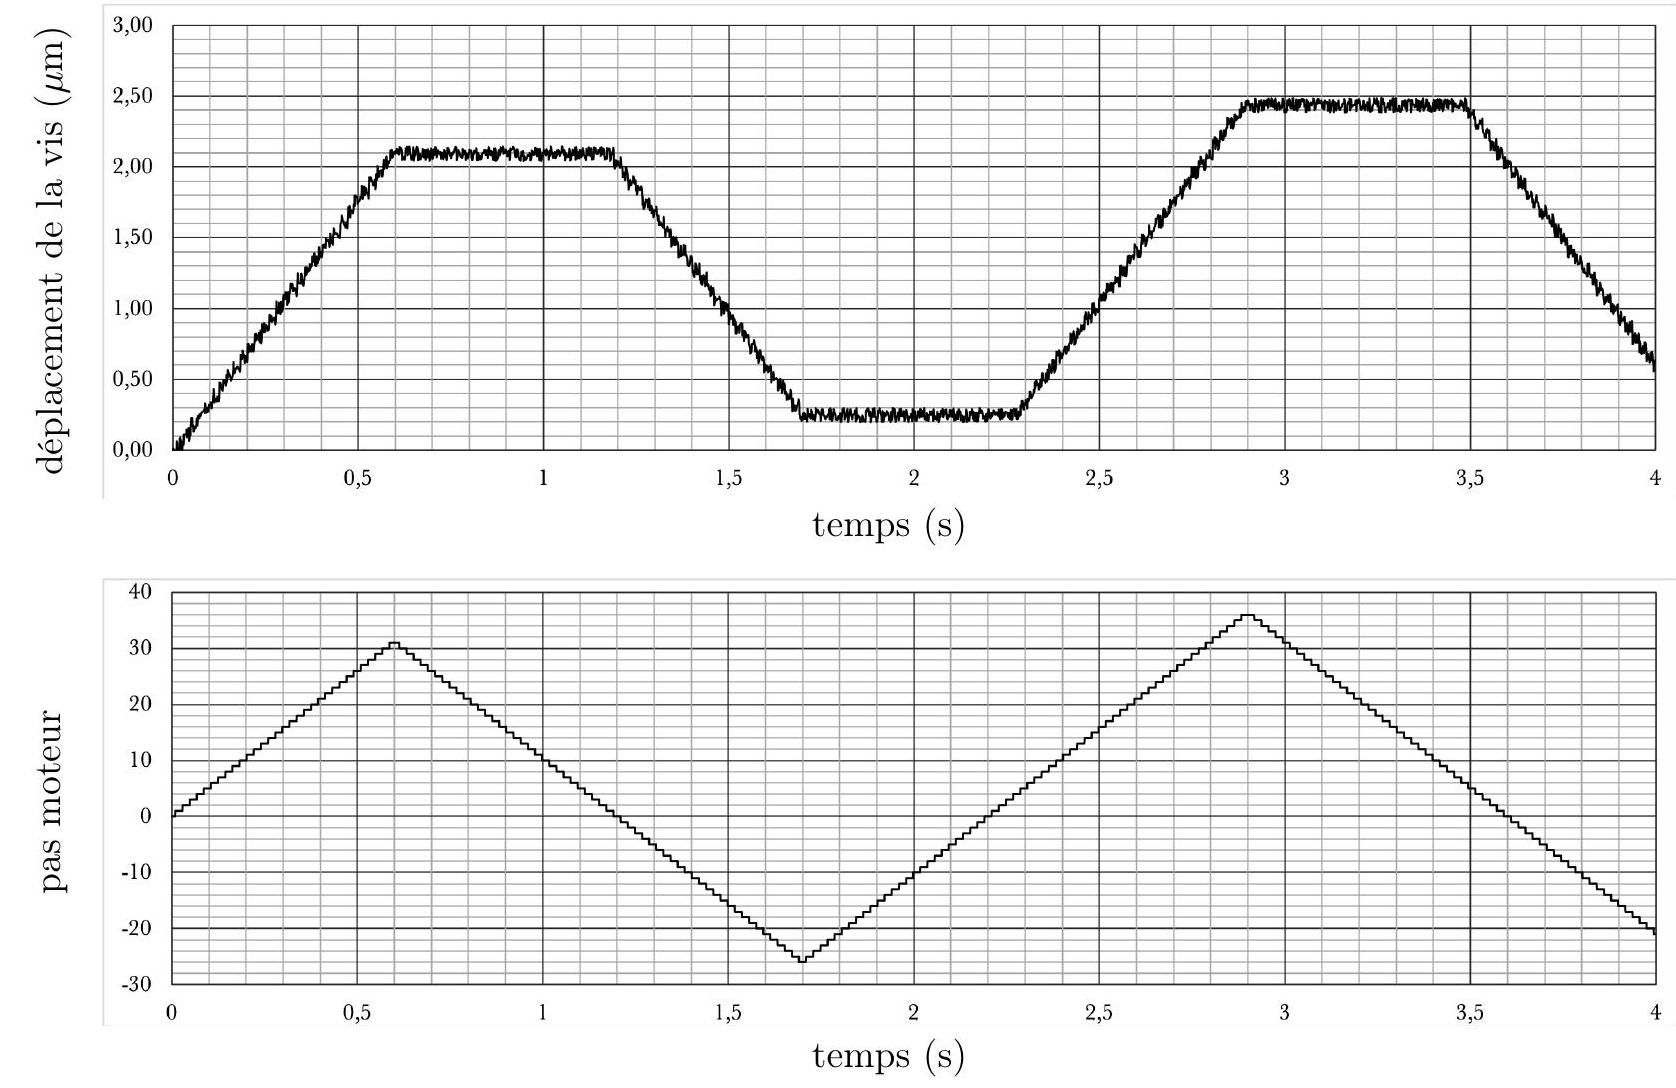
\includegraphics[width=\textwidth]{2024_04_26_3285cfc264024262add0g-08(1)}
\caption{\label{ccmp2023_fig_10} Déplacement de la vis en $\mu \mathrm{m}$ et nombre de pas du moteur en fonction du temps}
\end{figure}
%FigURe 10 - Déplacement de la vis en $\mu \mathrm{m}$ et nombre de pas du moteur en fonction du temps

\question{\label{ccmp2023_q_10}Proposer une cause de la non-linéarité qui apparait au changement de sens de rotation du moteur.}

\question{\label{ccmp2023_q_11}Donner l'erreur de positionnement due à la non-linéarité. Conclure à nouveau vis-à-vis de l'exigence 1.1 de précision du positionnement du centre d'inertie.}

